
    \documentclass[tikz,convert={outfile=\jobname.png}]{standalone}
    \usetikzlibrary{mindmap,trees,backgrounds}
    \usepackage{fontspec}
    \defaultfontfeatures{Ligatures=TeX,Scale=3}
    \setmainfont{M+ 1mn}
    
    
    \definecolor{60_174_163}{RGB}{60, 174, 163}
    \definecolor{244_208_63}{RGB}{244, 208, 63}
    \definecolor{250_215_160}{RGB}{250, 215, 160}
    \definecolor{169_50_38}{RGB}{169, 50, 38}
    \definecolor{118_68_138}{RGB}{118, 68, 138}
    \definecolor{156_100_12}{RGB}{156, 100, 123}
    \definecolor{229_152_102}{RGB}{229, 152, 102}
    \definecolor{black}{RGB}{0.0, 0.0, 0.0}
    \definecolor{darkgray}{RGB}{168.3, 168.3, 168.3}
    \definecolor{white}{RGB}{255.0, 255.0, 255.0}
    
    \begin{document}
    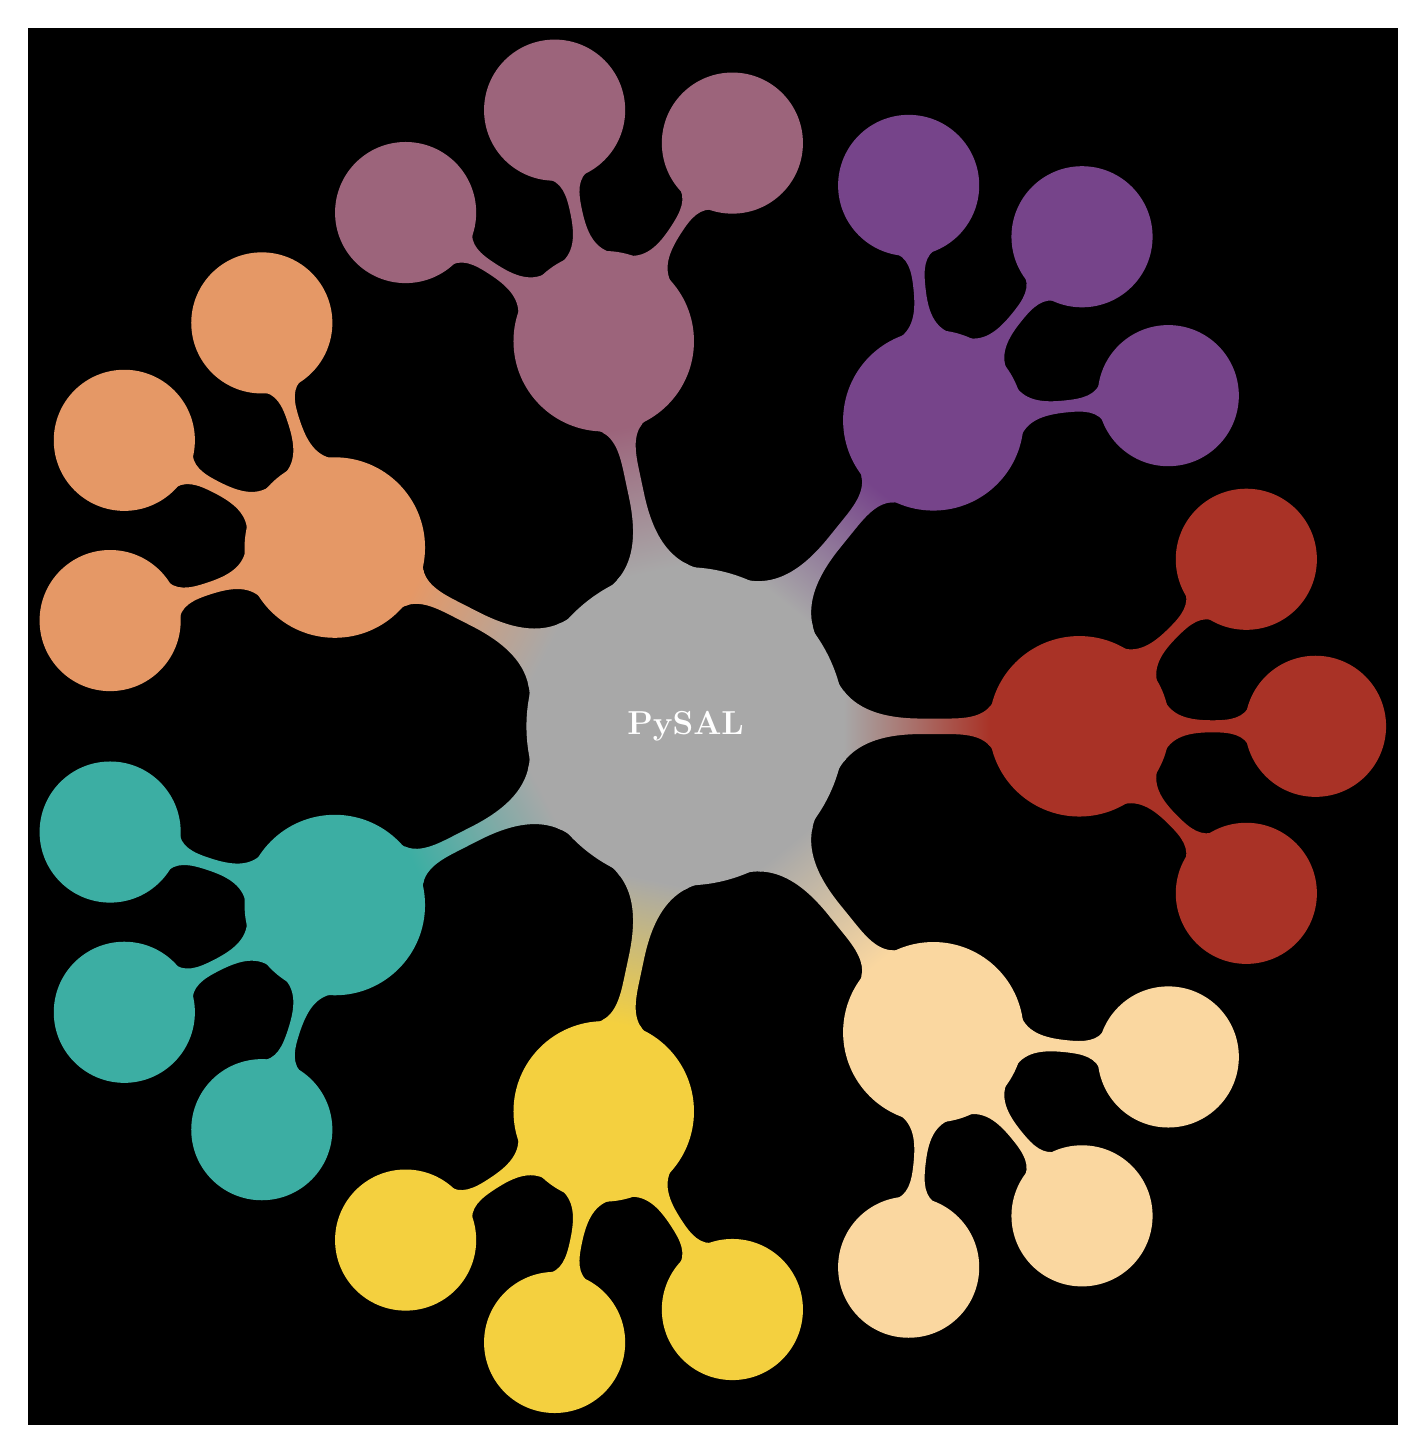
\begin{tikzpicture}[
        background rectangle/.style={fill=black},
        show background rectangle,
        mindmap,
        grow cyclic,
        every node/.style=concept,
        concept color=darkgray,
        text=white,
        level 1/.append style={
            level distance=5cm,
            sibling angle=51,
            font=\Huge
        },
        level 2/.append style={
            level distance=3cm,
            sibling angle=45
        }
    ]
    
        \node[concept color=darkgray]{\large\bfseries{PySAL}}
        child [concept color=60_174_163]{ node {}
            child { node { }}
            child { node { }}
            child { node { }}
         }
        child [concept color=244_208_63]{ node {}
            child { node { }}
            child { node { }}
            child { node { }}
         }
        child [concept color=250_215_160]{ node {}
            child { node { }}
            child { node { }}
            child { node { }}
         }
        child [concept color=169_50_38]{ node {}
            child { node { }}
            child { node { }}
            child { node { }}
         }
        child [concept color=118_68_138]{ node {}
            child { node { }}
            child { node { }}
            child { node { }}
         }
        child [concept color=156_100_12]{ node {}
            child { node { }}
            child { node { }}
            child { node { }}
         }
        child [concept color=229_152_102]{ node {}
            child { node { }}
            child { node { }}
            child { node { }}
         }
                ;
    \end{tikzpicture}
    \end{document}